\documentclass[a4paper]{article}

\usepackage{amssymb}
\usepackage{amsmath}
\usepackage{bm}

\numberwithin{equation}{subsection}

\usepackage{float}
\usepackage{array}
\usepackage{booktabs}
\usepackage{rotating}

\usepackage[margin=2cm, bottom=2cm, top=2cm, marginpar=0pt]{geometry}
\usepackage{graphicx}
\usepackage{xcolor}

%\usepackage{showframe}

%\usepackage{tikz}
%\usepackage{tikz-3dplot}
%\usepackage{pgfplots}
%\pgfplotsset{compat=1.15}

\usepackage{multicol}

\usepackage[colorlinks = true,
            linkcolor = red!50!black,
            urlcolor  = blue,
            citecolor = black,
            anchorcolor = blue]{hyperref}


\usepackage{polyglossia}
\setdefaultlanguage[variant=swiss]{german}


\title{Analysis 2 Zusammenfassung}
\author{Naoki Pross}
\date{Fr\"uhlingsstemester 2020}


\newcommand{\dd}[1]{\ensuremath{~\mathrm{d}#1}}
\newcommand{\deriv}[2]{\ensuremath{\frac{\dd{#1}}{\dd{#2}}}}
\newcommand{\pderiv}[2]{\ensuremath{\frac{\partial#1}{\partial#2}}}
\renewcommand{\vec}[1]{\ensuremath{\bm{#1}}}

\newcommand{\brpage}[1]{\textcolor{red!70!black}{\small\texttt{S#1}}}

\begin{document}

\begin{multicols}{2}
\section{Integration \brpage{493,507}}
\subsection{Tricks \brpage{495}}
Linearit\"at \brpage{495}
\[
	\int k(u + v) = k\left(\int u + \int v\right)
\]
Partialbruchzerlegung \brpage{15,498}
\[
	\int \frac{f(x)}{P_n(x)} \dd{x} = \sum_{k=1}^n \int \frac{A_k}{x-r_k}\dd{x}
\]
Elementartransformation \brpage{496}
\[
	\int f(\lambda x + \ell) \dd{x} = \frac{1}{\lambda} F(\lambda x + \ell) + C
\]
Partielle Integration \brpage{497}
\[
	\int u \dd{v} = uv - \int v \dd{u}
\]
Potenzenregel \brpage{496}
\[
	\int u^n \cdot u' = \frac{u^{n+1}}{n+1} + C \qquad n \neq -1
\]
Logaritmusregel \brpage{496}
\[
	\int \frac{u'}{u} = \ln|u| + C
\]
Allgemeine Substutution \brpage{497}\\
 \(x = g(u)\), und \(\dd{x} = g'(u)\dd{u}\)
\[
	\int f(x) \dd{x} = \int (f\circ g) ~ g' \dd{u} = \int \frac{f \circ g}{(g^{-1})'\circ g} \dd{u} 
\]
Universalsubstitution \brpage{504}
\begin{align*}
	t &= \tan(x/2) & \sin(x) &= \frac{2t}{1+t^2} \\
	\dd{x} &= \frac{2\dd{t}}{1+t^2} & \cos(t) &= \frac{1-t^2}{1+t^2} 
\end{align*}
Womit
\[
	\int f(\sin(x), \cos(x), \tan(x)) \dd{x} = \int g(t) \dd{t}
\]

\subsection{Uneigentliches Integral \brpage{520}}
\begin{align*}
	\int\limits_a^\infty f \dd{x} &= \lim_{B \to \infty} \int\limits_a^B f \dd{x} \\
	\int\limits_{-\infty}^b f \dd{x} &= \lim_{A \to -\infty} \int\limits_A^b f \dd{x} \\
	\int\limits_{-\infty}^\infty f \dd{x} &= \lim_{\substack{A \to +\infty \\ B \to -\infty}} \int\limits_A^B f \dd{x}
\end{align*}
Wenn \(f\) im Punkt \(u \in (a,b)\) nicht definiert ist.
\begin{equation} \label{eqn:int-with-pole}
	\int\limits_a^b f \dd{x} = 
	\lim_{\epsilon\to +0} \int\limits_a^{u-\epsilon} f \dd{x}
	+ \lim_{\delta\to +0} \int\limits_{u+\delta}^b f \dd{x}
\end{equation}

\subsection{Cauchy Hauptwert \brpage{523}}
Der C.H. (oder PV f\"ur \emph{Principal Value} auf Englisch) eines uneigentlichen Integrals ist der Wert, wenn in einem Integral wie \eqref{eqn:int-with-pole} beide Grenzwerte mit der gleiche Geschwindigkeit gegen 0 sterben.
\[
	\text{C.H.} \int\limits_a^b f \dd{x} = 
	\lim_{\epsilon\to +0} \left( \int\limits_a^{u-\epsilon} f \dd{x}
	+ \int\limits_{u+\epsilon}^b f \dd{x} \right)
\]
Zum Beispiel \(x^{-1}\) ist nicht \"uber \(\mathbb{R}\) integrierbar, wegen des Poles bei 0. Aber intuitiv wie die Symmetrie vorschlagt
\[
 	\text{C.H.} \int\limits^\infty_{-\infty} \frac{1}{x} \dd{x} = 0
\]

\subsection{Majorant-, Minorantenprinzip und Konvergenzkriterien \brpage{521,473,479,481}}

Gilt f\"ur die Funktionen \(0 < f(x) \leq g(x)\) mit \(x \in [a,\infty)\)
\[
	\text{konvergiert } \int\limits_a^\infty g \dd{x} 
	\implies \text{ konvergiert } \int\limits_a^\infty f \dd{x}
\]
Die selbe gilt umgekehrt f\"ur Divergenz. Wenn \(0 < h(x) \leq f(x)\) 
\[
	\text{divergiert } \int\limits_a^\infty h \dd{x} 
	\implies \text{ divergiert } \int\limits_a^\infty f \dd{x}
\]
\(g\) und \(h\) hei{\ss}en Majorant und Minorant bzw.

\section{Implizite Ableitung \brpage{448}}
Alle normale differenziazionsregeln gelten.
\[
	\dd{y} = y'\dd{x}
\]
%Allgemeiner f\"ur die implizite Funktion \(F(x,y) = 0\)
%\[
%	\pderiv{F}{x} + \pderiv{F}{y} y' = 0
%\]

\end{multicols}

\section{Ebene \brpage{250} und Raumkurven \brpage{263}}
\begin{sidewaystable}
\centering
\renewcommand{\arraystretch}{3}
\begin{tabular}{l *{3}{>{\(\displaystyle}l<{\)}} }
\toprule
\textbf{Ebene Kurven} & \textbf{Explizit } y = f(x) & \textbf{Polar } \vec{r}(\varphi) & \textbf{Parameter } \vec{c}(t) = \left(x(t), y(y)\right) \\
\midrule
Bogenl\"ange \brpage{251}
	& \int\limits_a^b \sqrt{1 + (f')^2} \dd{x}
	& \int\limits_\alpha^\beta \sqrt{(r')^2 + r^2} \dd{\varphi}
	& \int\limits_{t_0}^{t_1} \sqrt{\dot{x}^2 + \dot{y}^2} \dd{t} = \int\limits_{t_0}^{t_1} |\vec{c}| \dd{t}
\\
Fl\"ache
	& \int\limits_a^b |f(x)| \dd{x}
	& \frac{1}{2}\int\limits_\alpha^\beta r(\varphi)^2 \dd{\varphi}
	& \frac{1}{2}\int\limits_{t_0}^{t_1} x\dot{y} - \dot{x}y \dd{t} = \frac{1}{2}\int\limits_{t_0}^{t_1}\det(\vec{c},\dot{\vec{c}}) \dd{t}
\\
\midrule
Rotationsvolumen um \(x\)
	& \pi \left|\int\limits_a^b y^2 \dd{x} \right|
	& \pi \left|\int\limits_{t_0}^{t_1} y \dot{x} \dd{t} \right|
	& \pi \left|\int\limits_\alpha^\beta r^2 \sin^2 \varphi (r'\cos\varphi - r\sin\varphi) \dd{\varphi} \right|
\\
Rotationsoberfl\"ache um \(x\)
	& 2\pi \int\limits_a^b |y| \sqrt{1 + (y')^2} \dd{x}
	& 2\pi \int\limits_\alpha^\beta |r\sin(\varphi)| \sqrt{(r')^2 + r^2} \dd{\varphi}
	& 2\pi \int\limits_{t_0}^{t_1} |y| \sqrt{\dot{x}^2 + \dot{y}^2} \dd{t}
\\
% Rotationsvolumen um \(y\) \\
% Rotationsoberfl\"ache um \(y\) \\
\midrule
Kr\"ummung \(\kappa\)
	& \frac{f''}{\sqrt{1+(f')^2}^3}
	& 
	& \frac{\ddot{y}\dot{x} - \ddot{x}\dot{y}}{\sqrt{\dot{x}^2 + \dot{y}^2}^3} 
	= \frac{\det(\vec{\dot{c}},\vec{\ddot{c}})}{|\vec{\dot{c}}|^3}
\\
\bottomrule
\end{tabular}
\end{sidewaystable}

\begin{multicols}{2}
\subsection{Darstellungen}
\begin{figure}[H]
\centering
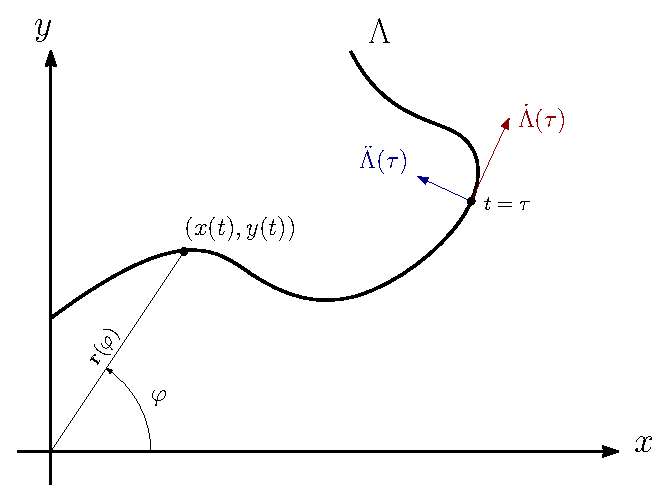
\includegraphics[width=.9\linewidth]{fig/plane-curve.eps}
\caption{Die ebene Kurve \(\Lambda(t)\) kann Explizit \(y(x)\) (in diesem Fall nicht), Implizit \(\vec{u}(x,y)\), Polar \(\vec{r}(\varphi)\) oder in Parameterform \((x(t), y(t))\) dargestellt werden.}
\end{figure}

\subsection{Tangente und Normalvektor}

\subsection{Kr\"ummung}
\[
	\kappa = \deriv{\phi}{s} = \frac{\ddot{y}}{(1+\dot{y}^2)^{3/2}}
\]

\begin{thebibliography}{1}
  \bibitem{hsr}
    \texttt{An2E} Vorlesungen an der Hochschule f\"ur Technik Rapperswil und der dazugeh\"orige Skript,
    \textit{Dr. Bernhard Zgraggen}, Fr\"uhlingssemester 2020
  \bibitem{bronstein}
    Taschenbuch der Mathematik,
    10. \"uberarbeitete Auflage, 2016 (1977),
    \textit{Bronstein, Semendjajew, Musiol, M\"uhlig}, 
    \texttt{ISBN 978-3-8085-5789-1}
  \bibitem{mathe2}
    Mathematik 2 Lehrbuch für ingenieurwissenschaftliche Studieng\"ange,
    2012, 7. Auflage, XII, Springer Berlin,
    \textit{Albert Fetzer, Heiner Fränkel},
    \texttt{ISBN-10 364224114X},
    \texttt{ISBN-13 9783642241147}
    
\end{thebibliography}

\section*{Notation}
Rot markierte Zahlen wie zB \brpage{477} sind Hinweise auf die Seiten im ``Bronstein'' \cite{bronstein}

\section*{License}
{ \tt
An2E-ZF (c) by Naoki Pross
\\\\
An2E-ZF is licensed under a Creative Commons Attribution-ShareAlike 4.0 Unported License.
\\\\
You should have received a copy of the license along with this work. If not, see 
\\\\
\url{http://creativecommons.org/licenses/by-sa/4.0/}
}

\end{multicols}
\end{document}